\documentclass[11pt,a4paper]{article}
\usepackage[hyperref]{acl2020}
\usepackage{booktabs}
\usepackage{graphicx}
\usepackage{times}
\usepackage{latexsym}
\renewcommand{\UrlFont}{\ttfamily\small}

\usepackage{microtype}

\aclfinalcopy % Uncomment this line for the final submission


\newcommand\BibTeX{B\textsc{ib}\TeX}

\title{Using Natura Language Processing to Identify Unfair Clauses in Terms and Conditions Documents}

\author{Jonathan Sears\\
  Tulane University / New Orleans, LA \\
  \texttt{jsears1@tuane.edu} \\\And
  Nicholas Radwin \\
  Tulane  / New Orleans, LA\\
  \texttt{nradwin@tulane.edu} \\}

\date{}

\begin{document}
\maketitle



\section{Problem Overview}

No one reads Terms and Conditions, but everyone agrees to them. Every online user is faced with these incredibly dense and complex documents as if they are expected to read them in their entirety before using a digital tool or app that they want to use. In reality, we just agree to the terms and conditions to use what's behind them, leaving the user in the dark from the ambiguous, unfair, and even potentially exploitative clauses that may not be in the user's best interest.

Our project is focused on bringing these buried, questionable clauses to light so that the user can understand what he is agreeing to at a glance. As we experiment with a variety of learning models, we are building a summarization tool that takes in terms and conditions as input and generates a page that bullets a list of either ambiguous, unfair, or exploitative clauses with a confidence score for how likely the model chose those sentences correctly. We also want the tool to highlight the sentences from the original text.

\section{Data}

Our labeled data comes from a repository called PileOfLaw (link 1 below), which is full of ~256GB of legal and administrative documents in the English language.
Within PileOfLaw, there are two pretrained BERT models which differ only in seed. We decided to use the second model (link 2 below), as it is the same seed used in the original paper that used PileOfLaw; that way we can compare results to get better insight into how well any modifications we make are performing.
https://huggingface.co/datasets/pile-of-law/pile-of-law
https://huggingface.co/pile-of-law/legalbert-large-1.7M-2


\section{Methods}

What method or algorithm are you using. 
Are you using an existing library to do so? 
Did you introduce any new variations to these methods? 
How will you evaluate the results? 
Which baselines will you compare against?


\section{Preliminary Experiments and Results}

State and evaluate your results up to the milestone.

Table~\ref{tab:a_table} shows a table. Note that we refer to output generated by \texttt{Experiments.ipynb}. This way, whenever we re-run our notebook, we can regenerate the paper with the latest results.

\begin{table}[ht]
\centering
% note that we can refer to tables generated by our Experiments.ipynb notbook.
\begin{tabular}{rr}
\toprule
    C &    F1 \\
\midrule
  0.1 &  0.90 \\
  1.0 &  0.92 \\
  5.0 &  0.93 \\
 10.0 &  0.89 \\
\bottomrule
\end{tabular}

\caption{\label{tab:a_table} A caption. }
\end{table}

Figure~\ref{fig:a_label} shows a figure

\begin{figure}[ht]
	\centering
	% note that we can refer to figures generated by our Experiments.ipynb notbook.
	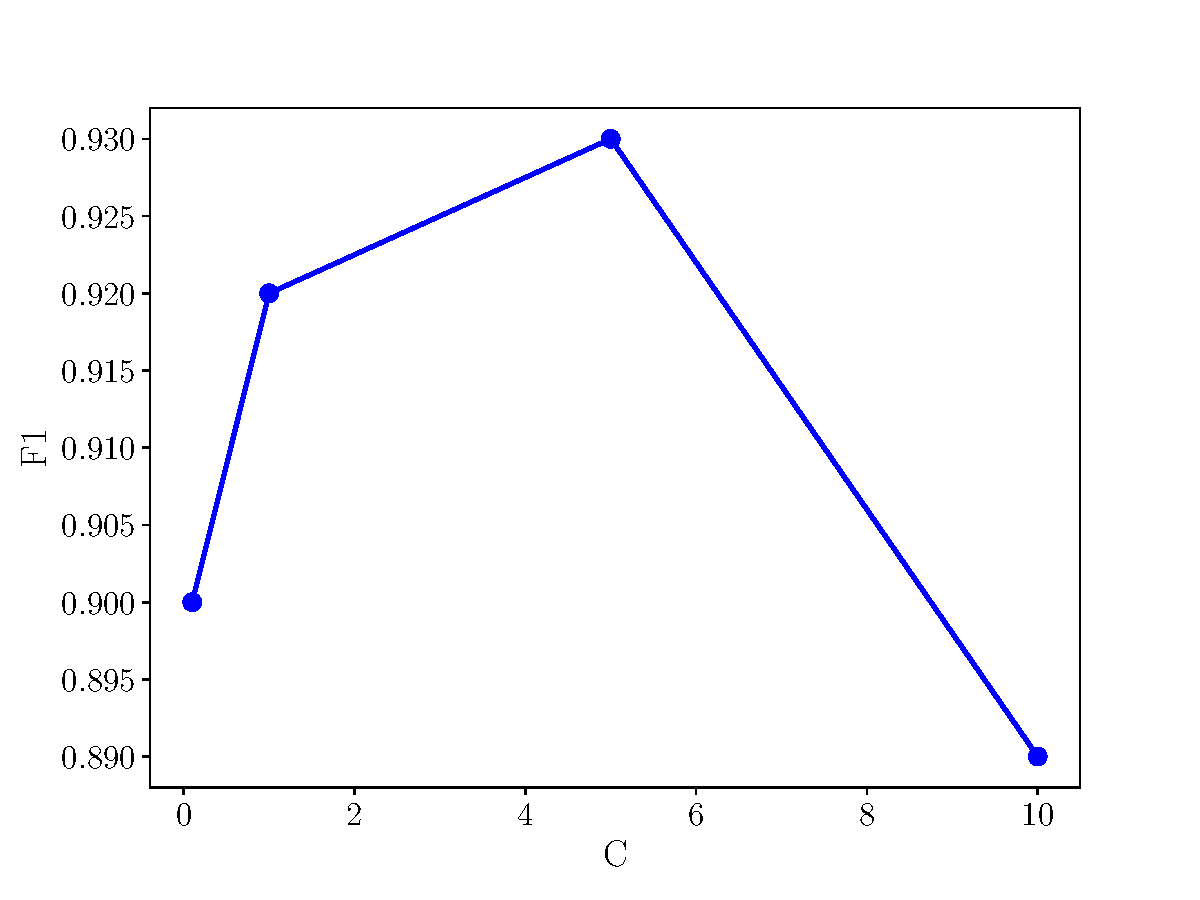
\includegraphics[width=3.5in]{../notebooks/results.pdf}
	\caption{A caption}
	\label{fig:a_label}
\end{figure}

\section{Related Work}

Citations within the text appear in parentheses as~\citep{aho1972theory} or, if the author's name appears in the text itself, as \citet{andrew2007scalable}.

1. CLAUDETTE
https://arxiv.org/pdf/1805.01217v2.pdf

CLAUDETTE is an automated detector of potentially unfair clauses in terms and conditions, basically exactly what we are trying to build. The data they used was 50 annotated European terms of service contracts. It is worth noting they used European contracts, as different countries mean different laws, and different language used in the contracts. They used a wide variety of different ML approaches to this problem including, support vector machines, hidden markov models, LSTMs, CNNs, and different combinations of them, getting the best results (measured in F1-score) via the combined model.  

2. Detecting and explaining unfairness in consumer contracts through memory networks
https://link.springer.com/article/10.1007/s10506-021-09288-2

In this study, the researchers define unfair legal language in terms and conditions as language that causes "a significant imbalance in the parties' rights and obligations, to the detriment of the consumer, are deemed unfair by Consumer Law."

They note how pervasive this point out that despite substantive law in place, and despite the competence of enforcers, providers of online services still tend to use unfair and unlawful clauses in these documents."

Their system is trained on 100 labeled ToS documents and is based on splitting unfair clauses into 5 major label categories:

(i) liability exclusions and limitations

(ii) the provider’s right to unilaterally remove consumer content from the service, including in-app purchases

(iii) the provider’s right to unilaterally terminate the contract

(iv) the provider’s right to unilaterally modify the contract and/or the service

(v) arbitration on disputes arising from the contract

The unfair language/rationale pairing output was most accurate when the researchers used a memory-augmented neural network in combination with "strong supervision," meaning that they fed the expertly written rationales for specific unfair labels into their model.

3. LexGLUE: A Benchmark Dataset for Legal Language Understanding in English
chrome-extension://efaidnbmnnnibpcajpcglclefindmkaj/https://aclanthology.org/2022.acl-long.297.pdf

The LexGLUE paper was written to create a benchmark for legal language understanding. It is a compilation of datasets, pretrained models and different tests and evaluation metrics performed on those datasets and models for different tasks. We think it will be useful as both a potential source and potential benchmark for our model.

4. Automatic semantics extraction in law documents
https://dl.acm.org/doi/10.1145/1165485.1165506 

This study aimed to classify arguments from legislative texts using the multiclass support vector machine (MSVM) algorithm.

Stemming (representing the morphology/roots of words) improved accuracy and feature selection (restricted vocabulary) provided a work around for possible overfitting.

Overall, the study showcases MSVM's effectiveness in extracting what arguments are actually being made in legal documents,
and helps us with coming up with a method for efficient legal document analysis.

5. When Does Pretraining Help? Assessing Self-Supervised Learning for Law and the CaseHOLD Dataset
https://arxiv.org/abs/2104.08671

This paper presents an argument for domain specific pretraining and tests it's hypothesis on a dataset of their own creation: CaseHOLD. They compare the performance of wide domain BERT models trained separately on a corpus of legal documents (smaller, specific domain) and another model trained on wikipedia and google books (wider domain). They found that pretraining on the smaller corpus of legal documents was more effective for legal classification tasks despite their being much less data available. This leads us to believe that if we decide to use a pretrained model, we will likely use one that is domain specific to legal documents. 

Since our problem is a classification problem, we think an 80-20 cross validation approach with metrics like our accuracy, precision, recall, and F1 score should suffice. However, the scale in which we perform these evaluation metrics may vary, as we may want to measure them on a document level, and on a sentence by sentence level. We can use pretrained models, as well as a simple logistic regression and naïve Bayes models as baseline metrics to compare our model too. 

\section{Division of Labor}
State which group member is responsible for which aspects of the project.

\section{Timeline}
What are the remaining steps you plan to complete, and when do you plan to complete them?


\bibliography{references}
\bibliographystyle{acl_natbib}
@misc{hendersonkrass2022pileoflaw,
  url = {https://arxiv.org/abs/2207.00220},
  author = {Henderson, Peter and Krass, Mark S. and Zheng, Lucia and Guha, Neel and Manning, Christopher D. and Jurafsky, Dan and Ho, Daniel E.},
  title = {Pile of Law: Learning Responsible Data Filtering from the Law and a 256GB Open-Source Legal Dataset},
  publisher = {arXiv},
  year = {2022}
}
@inproceedings{drawzeski-etal-2021-corpus,
  address = {Punta Cana, Dominican Republic},
  author = {Drawzeski, Kasper and Galassi, Andrea and Jablonowska, Agnieszka and Lagioia, Francesca and Lippi, Marco and Micklitz, Hans Wolfgang and Sartor, Giovanni and Tagiuri, Giacomo and Torroni, Paolo},
  booktitle = {Proceedings of the Natural Legal Language Processing Workshop 2021},
  doi = {10.18653/v1/2021.nllp-1.1},
  month = {nov},
  pages = {1--8},
  publisher = {Association for Computational Linguistics},
  title = {{A Corpus for Multilingual Analysis of Online Terms of Service}},
  url = {https://aclanthology.org/2021.nllp-1.1},
  year = {2021}
}
@misc{hendersonkrass2022pileoflaw,
  url = {https://arxiv.org/abs/2207.00220},
  author = {Henderson, Peter and Krass, Mark S. and Zheng, Lucia and Guha, Neel and Manning, Christopher D. and Jurafsky, Dan and Ho, Daniel E.},
  title = {Pile of Law: Learning Responsible Data Filtering from the Law and a 256GB Open-Source Legal Dataset},
  publisher = {arXiv},
  year = {2022}
}

\end{document}
